\section{Verificatie}

%inleiding over welke testen we gaan uitvoeren en waarom. Over hoe de testen zijn opgesteld en wat het doel is van de totaliteit testen.

\subsection{Enkele communicatie Test}
% uitleg wat de test is met doel
Deze test kijkt naar de communicatie tussen twee nodes. Het doel is om te kijken hoe betrouwbaar de connectie is en 
over welke afstand de communicatie nog steeds betrouwbaar is. De test zal beginnen door eerst 100 berichten naar de andere 
node te sturen op een afstand van 10 cm en te kijken hoeveel van de berichten aankomt bij de andere node. Zo zal na elke test de 
afstand worden vergroot totdat de betrouwbaarheid onder de 90\% komt. Daarna is de kans dat een bericht voor onze specificaties te 
klein en op deze manier weten we ook meteen hoever de nodes van elkaar af moeten staan. De betrouwbaarheid wordt gebasseerd op de 
hoeveelheid aan berichten dat is aangekomen van de 100 berichten. Daarnaast wordt ook de trust levels vastgelegd 
die het systeem zelf meet. Dit wordt gedaan om de data met elkaar te vergelijken en hier conclusies aan vast te leggen.
% Test opstelling
In onderstaande afbeelding \ref{fig:TestCom} is de testopstelling opgezet. Te zien is dat er twee xmega's nodig zijn met een NRF chip. 
Deze moeten naar elkaar kijken en worden na elke test met afstand vergroot. Bij deze test zal er niks tussen de verbinding zitten.
\begin{figure}[h]
    \centering
    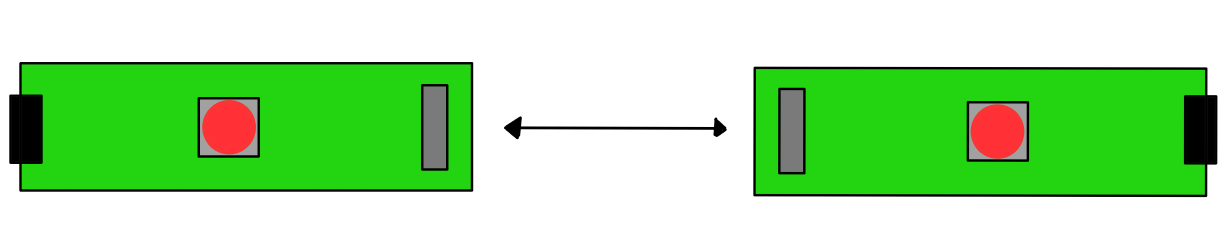
\includegraphics{img/Screenshot_292.png}
    \caption{Test opstelling}
    \label{fig:TestCom}
\end{figure}
% Randvoorwaarden 
De test is pas voltooid wanneer de grootste betrouwbaarheid met de grootste afstand mogelijk gevonden is. Dit moet een directe 
lijn zijn zonder obstakels tussen de nodes. de betrouwbaarheid moet boven de ...\% liggen zoals beschreven in de specificaties.
% Resultaten test
In onderstaande tabel \ref{Test:EnkelCom} zijn de testreulstaten te zien.
\begin{table}[h]
    \centering
    \begin{tabular}{|c||c|c|c|c|}
        \hline
        Test    & Afstand   & Aangekomen berichten  & Trust & Betrouwbaarheid   \\\hline\hline
        Test 1  & 10 cm     &                       &       &                   \\\hline
        Test 2  & 15 cm     &                       &       &                   \\\hline
        Test 3  & 20 cm     &                       &       &                   \\\hline
        Test 4  & 30 cm     &                       &       &                   \\\hline
        Test 5  & 50 cm     &                       &       &                   \\\hline
        Test 6  & 100 cm    &                       &       &                   \\\hline
        Test 7  & 150 cm    &                       &       &                   \\\hline
        Test 8  & 200 cm    &                       &       &                   \\\hline   
    \end{tabular}
    \caption{Testresultaten Enkele communicatie Test}
    \label{Test:EnkelCom}
\end{table}
% Conclusie test

\subsection{Hop Test}
% uitleg wat de test is met doel
Deze test is vergelijkbaar met vorige test, maar maakt gebruik van één extra node tussen de twee versturende en ontvangende nodes. 
Het doel van deze test is om te kijken hoe betrouwbaar de hop communicatie is. Ook kan er gekeken worden op welke maximale afstand 
de hops ook nog steeds werken. 
% Test opstelling
Voor deze test zijn drie nodes nodig. In onderstaande afbeelding \ref{fig:Testhop} is te zien hoe de nodes moeten staan.
 Één die ontvangt, één die verstuurd en één die gebruikt wordt als hop. Ook voor deze test wordt er na elke test 
 de afstand tussen de nodes vergroot. Dit wordt per kant gedaan. Dus eerst vergroot de rechterkant met een kleine afstand 
en dan vergroot de linkerkant van de hop node tussen de andere node met een kleine afstand.

\begin{figure}[h]
    \centering
    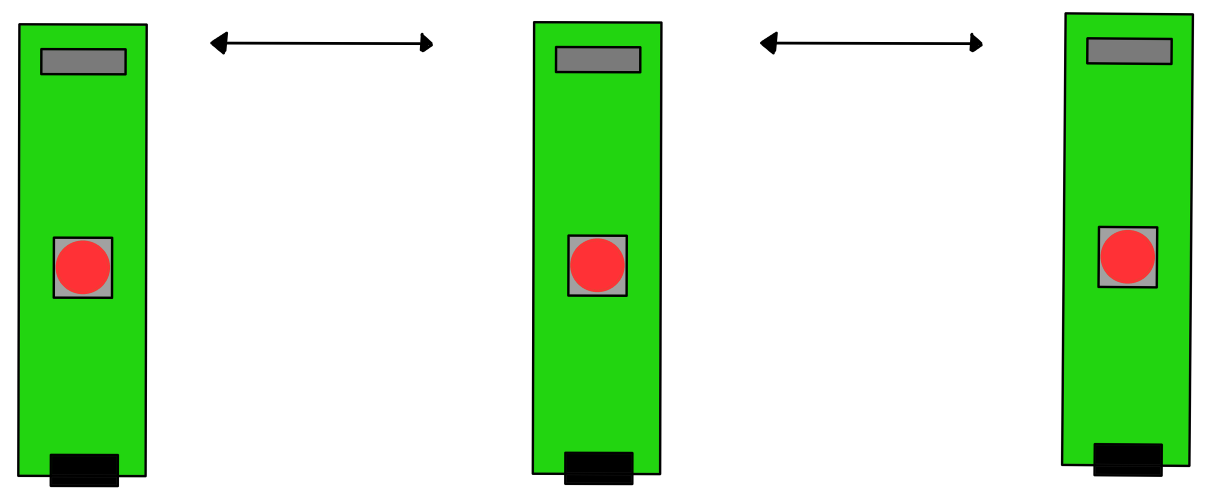
\includegraphics{img/Screenshot_293.png}
    \caption{Test opstelling 2}
    \label{fig:Testhop}
\end{figure}
% Randvoorwaarden
Deze test wordt pas als voltooid gezien wanneer de betrouwbaarheid boven de ...\% blijft liggen Met een zo groot mogelijke afstand 
tussen de nodes.
% Resultaten test
\begin{table}[h]
    \centering
    \begin{tabular}{|c||c|c|c|c|}
        \hline
        Test    & Afstand rechterkant  & Afstand linkerkant & Aangekomen berichten  & Trust & Betrouwbaarheid   \\\hline\hline
        Test 1  & 10 cm                & 10 cm              &                       &       &                   \\\hline
        Test 2  & 15 cm                & 10 cm              &                       &       &                   \\\hline
        Test 3  & 15 cm                & 15 cm              &                       &       &                   \\\hline
        Test 4  & 30 cm                & 15 cm              &                       &       &                   \\\hline
        Test 5  & 30 cm                & 30 cm              &                       &       &                   \\\hline
        Test 6  & 50 cm                & 30 cm              &                       &       &                   \\\hline
        Test 7  & 50 cm                & 50 cm              &                       &       &                   \\\hline
        Test 8  & 100 cm               & 50 cm              &                       &       &                   \\\hline
        Test 9  & 100 cm               & 100 cm             &                       &       &                   \\\hline 
        Test 10 & 200 cm               & 100 cm             &                       &       &                   \\\hline 
        Test 11 & 200 cm               & 200 cm             &                       &       &                   \\\hline   
    \end{tabular}
    \caption{Testresultaten Hop Test}
    \label{Test:Hop}
\end{table}

% Conclusie test

\subsection{Totale communicatie Test}
% uitleg wat de test is met doel
% Test opstelling
% Randvoorwaarden 
% Resultaten test
% Conclusie test

\subsection{Encryptie Test}
% uitleg wat de test is met doel
% Test opstelling
% Randvoorwaarden 
% Resultaten test
% Conclusie test

\subsection{Interface Test}
% uitleg wat de test is met doel
% Test opstelling
% Randvoorwaarden 
% Resultaten test
% Conclusie test